\subsection{Metodología de testeo}
A continuación se presenta un análisis comparativo de los tres métodos implementados.
Cabe mencionar que, dado que la experimentación requería que ambas imágenes (original y modificada) tengan el mismo tamaño para poder realizar un análisis cuantitativo de los algoritmos mediante las medidas de comparación que se mencionaron en la introducción, decidimos achicar la imagen original mediante un script que creamos para luego agrandarla mediante nuestros métodos y poder comparar los resultados obtenidos con la imagen original.

El recortador de imágenes, que se encuentra en la carpeta $\textsf{Recortador de imágenes}$, toma una imagen como input la cual se quiere achicar para poder comparar con si misma en tamaño original una vez aplicado el algoritmo de zoom y un entero $k$ que es el factor de achicamiento, que debe ser el mismo que usemos a la hora de aplicar zoom sobre esta imagen achicada. Este script lo hicimos utilizando $OpenCV$, de modo similar a las funciones utilizadas para hacer zoom en la experimentación base.

El comportamiento de este programa es sencillo, partiendo de una imagen original toma un pixel cada $k$ pixeles hasta llegar al final de la imagen. De esta manera, al aplicar los algoritmos de zoom, estas $k$ posiciones serán completados nuevamente y podremos comparar como completa cada método la imagen. Puede que algunas columnas del final queden truncadas ya que no siempre es posible partir una imagen perfectamente de esta manera, pero consideramos que esas pocas columnas son despreciables para una imagen lo suficientemente grande. 

Para asegurarnos que todos los cálculos sean lo mas precisos posibles utilizamos la extinción $.png$ para guardar todas las imágenes con as que trabajamos, ya que este formato utiliza un algoritmo de compresión sin pérdida que nos asegura que ninguna información se pierde al momento de guardar las imágenes.

\subsubsection{Artifacts}

Además de las métricas ya mencionadas brevemente en la introducción realizaremos un análisis visual de las imágenes y de los errores que se puedan percibir.

Para ello prestaremos atención a los artifacts que se puedan observar en las imágenes reconstruidas. Un artifact digital es un error no deseado o no intencionado en los datos debido a la manipulación de la información. Existen muchas causas por las cuales se pueden generar artifacts, desde algún desperfecto en el hardware, debido a la compresión de los datos, etc.

Además existen variados tipos de artifacts, a continuación describiremos algunos:

\begin{itemize}
 \item Ruido:
 \\
 	El ruido en imágenes digitales es mas claramente visible sobre superficies uniformes donde se pueden observar cierto tipo de granularidades.
 \item Aliasing:
 \\
 	El aliasing de una imagen puede describirse de manera informal como los 'serruchos' que pueden observarse cerca de los bordes de los objetos.
 \item Sharpening:
 \\
 El Sharpening ocurre cuando al agrandar una imagen se sobre dimensionan los bordes de tal manera que la imagen parezca tener mas contraste.
\end{itemize}
A continuación se muestra un ejemplo de cada uno de estas aberraciones:
\begin{figure}[H]
\centering
\subfloat[Ruido]{{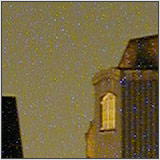
\includegraphics[width=3cm]{fotos/artifacts/ruido.jpg} }}
\qquad
\subfloat[Aliasing]{{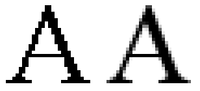
\includegraphics[width=3cm]{fotos/artifacts/aliasing.png} }}
\qquad
\subfloat[Sharpening]{{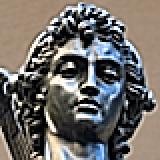
\includegraphics[width=3cm]{fotos/artifacts/sharp.png} }}
\caption{Artifacts}
\end{figure}

\subsection{Correctitud de la implementación}

El primer método para comprobar rápidamente la correctitud de la implementación de nuestros algoritmos fue sencillamente comparar ''a ojo'' las imágenes resultantes con la original, observando el nivel de detalle obtenido. Al comienzo, teniendo errores de implementación, notamos de este modo que la implementación necesitaba mejoras.

Luego, para obtener mayor rigor, procedimos a comparar nuestros algoritmos con aquellos que vienen por defecto en opencv. Consideramos que estos algoritmos son lo suficientemente fiables como para tomarlos como punto de referencia. Tomamos una imagen:
\begin{figure}[H]
    \centering
\subfloat[.]{{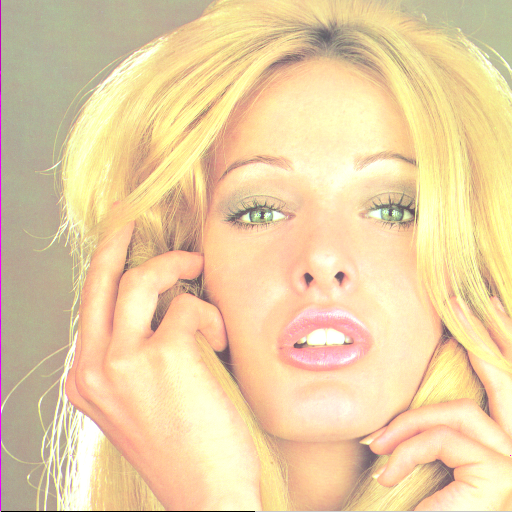
\includegraphics[width=5cm]{fotos/opencvvsus/orig.png} }}
\caption{Imagen Original}
\end{figure}
Y la reescalamos en la mismas dimensiones tanto con nuestros algoritmos como con los implementados en Opencv.

\begin{figure}[H]
    \centering
    \subfloat[Nosotros]{{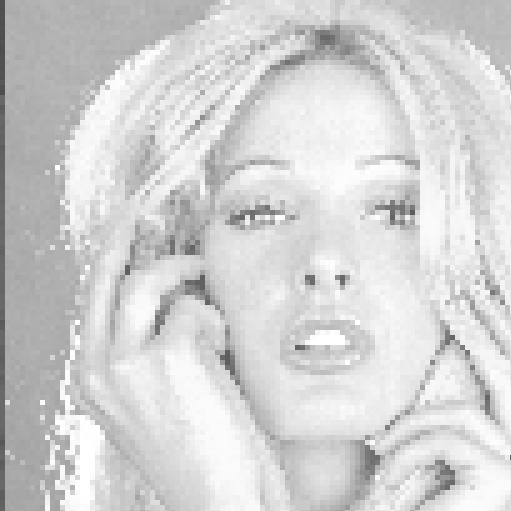
\includegraphics[width=5cm]{fotos/opencvvsus/1us.png} }}
    \qquad
    \subfloat[OpenCV]{{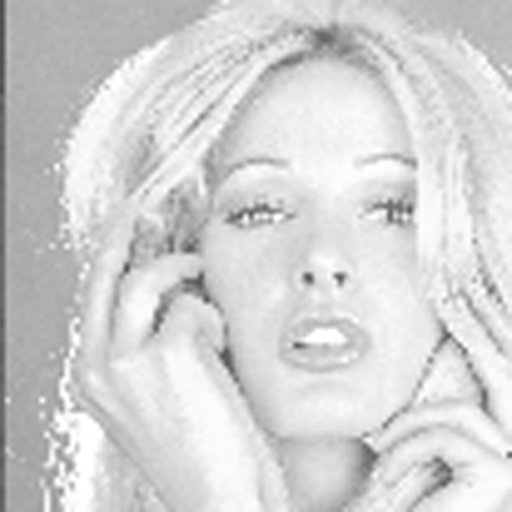
\includegraphics[width=5cm]{fotos/opencvvsus/1open.png} }}
    \caption{Comparación de correctitud contra Opencv: Vecinos Mas Cercanos}
\end{figure}

\begin{figure}[H]
    \centering
    \subfloat[Nosotros]{{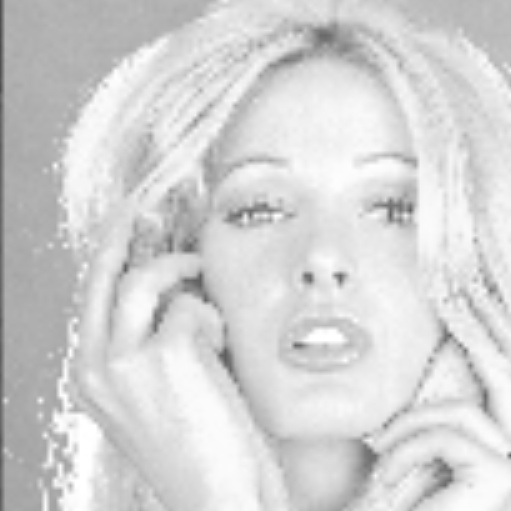
\includegraphics[width=5cm]{fotos/opencvvsus/2us.png} }}
    \qquad
    \subfloat[OpenCV]{{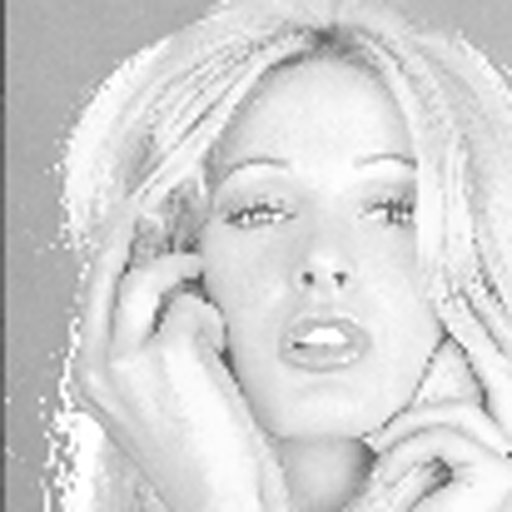
\includegraphics[width=5cm]{fotos/opencvvsus/2open.png} }}
    \caption{Comparación de correctitud contra Opencv: Bilineal}
\end{figure}

\begin{figure}[H]
    \centering
    \subfloat[Nosotros]{{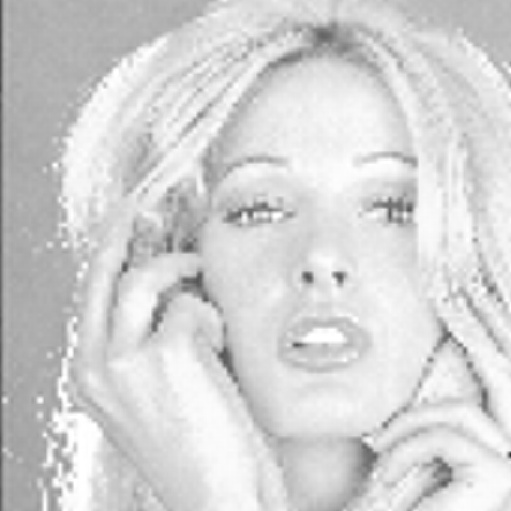
\includegraphics[width=5cm]{fotos/opencvvsus/3us.png} }}
    \qquad
    \subfloat[OpenCV]{{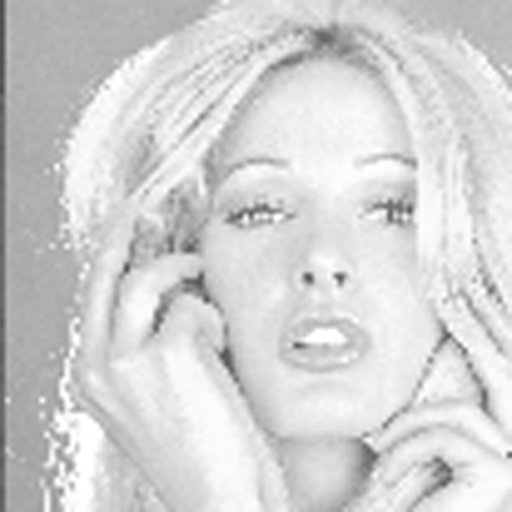
\includegraphics[width=5cm]{fotos/opencvvsus/3open.png} }}
    \caption{Comparación de correctitud contra Opencv: Bicubico con ventanas de $4\times4$ píxeles}
\end{figure}

Como puede verse, nuestros algoritmos arrojan resultados muy similares a Opencv. Por lo que consideramos que su implementación es correcta.

\subsection{Ventana óptima para método de Splines}
Nuestro primer análisis se encargará de encontrar un valor óptimo para la cantidad de las ventanas utilizadas en el método de splines.
Para dicho fin, elegimos correr varias instancias del método con valores de $K$ crecientes para distintos valores de ventana (4, 8, y 16 para poder comparar los resultados). Se presentan entonces los resultados obtenidos. Vale la pena destacar que no se muestra información respecto al PSNR debido a que presentaba exactamente el mismo comportamiento y no ofrecía información extra alguna.
\\
Como habíamos presupuesto en la introducción, agrandar el tamaño de la ventana solo hace que se tengan en cuenta valores para el punto que se quiere calcular que no depende directamente de este. 

\begin{center}
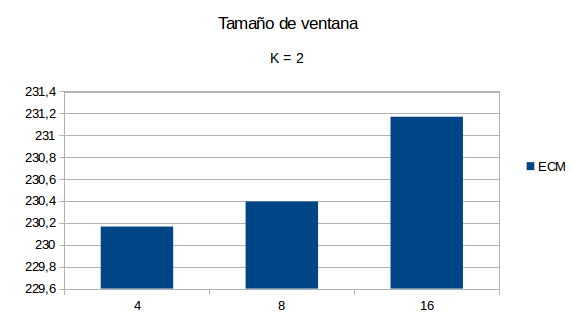
\includegraphics[scale=0.50]{imagenes/VK2.png}
\end{center}

Como puede verse a continuación, agrandar el tamaño de la ventana deja de presentar beneficio alguno para valores mas altos de $K$ porque los resultados se vuelven constantes:

\begin{center}
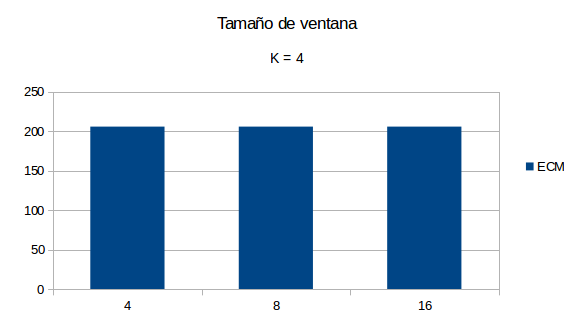
\includegraphics[scale=0.50]{imagenes/VK4.png}
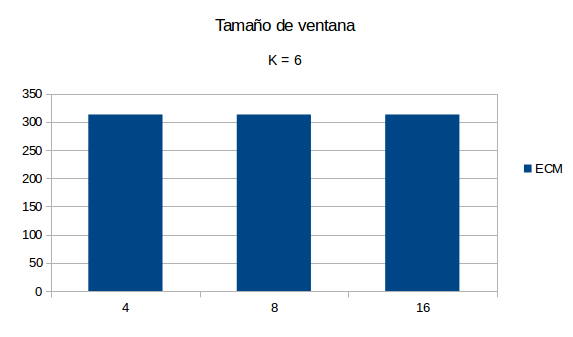
\includegraphics[scale=0.50]{imagenes/VK6.png}
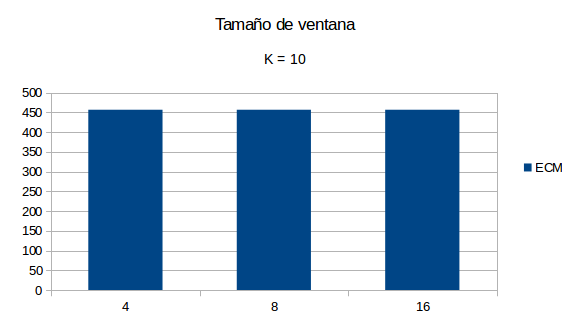
\includegraphics[scale=0.50]{imagenes/VK10.png}
\end{center}

A partir de este punto, el algoritmo de splines utiliza una ventana de tamaño cuatro, dado que es la que presenta mejores resultados.
De todos formas, no es cierto que siempre sea preferible una ventana más chica a una que incluya mas puntos, porque en problemas donde se quieren calcular por ejemplo trayectorias, es deseable considerar mas puntos para tener mas información.

\subsection{Análisis de los métodos}
\subsubsection{Análisis de los métodos para imágenes con símbolos alfanuméricos}
En esta sección analizaremos los tres algoritmos sobre imágenes con símbolos alfanuméricos. Para ellos usamos la imagen mostrada mas abajo para la cual aplicaremos los tres algoritmos implementados con diferentes ks.

Para ello, tomamos la imagen original de $256 \times 256$ y reducimos su tamaño de la manera ya mencionada al principio de esta sección. De esta manera al aplicarle el $k$ se obtiene un tamaño similar al original. Para este experimento, las imágenes reconstruidas a través de este procedimiento tendrán un tamaño entre $255 \times 255$ y $226 \times 256$.

La característica principal que querremos testear será la capacidad de discernimiento de estos símbolos después de aplicados los métodos de zoom.

\begin{figure}[H]
\centering
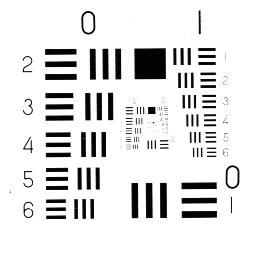
\includegraphics[scale=0.50]{fotos/alfanum/orig.png}
\end{figure}

Primero realizamos las pruebas con el valor mínimo de $k$ ($k=1$), obteniendo los siguientes resultados:


\begin{figure}[H]
    \centering
    \subfloat[Método 1]{{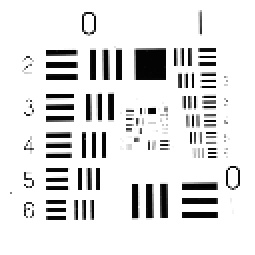
\includegraphics[width=5cm]{fotos/alfanum/k1_1.png} }}
    \qquad
    \subfloat[Método 2]{{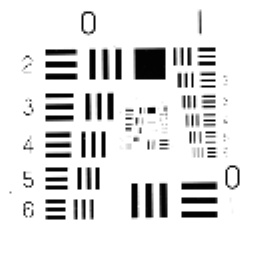
\includegraphics[width=5cm]{fotos/alfanum/k1_2.png} }}
    \qquad
    \subfloat[Método 3]{{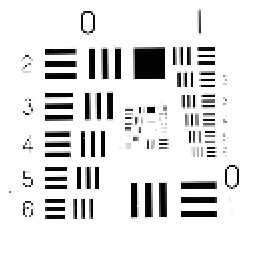
\includegraphics[width=5cm]{fotos/alfanum/k1_3.png} }}
    \caption{Comparación de métodos para $k = 1$}
    \label{fig:example}
\end{figure}

Como podemos ver, las tres imágenes introducen artifacts que todavía no desmejoran la imagen a un nivel en el que sea imposible su comprensión, por lo menos en los dígitos mas externos (distinto para los números internos de la imagen que, debido a su tamaño inicial, ya son casi imperceptibles con este $k$ mínimo). Notese como el método $2$ (el algoritmo bilineal), como consecuencia de la nivelación entre los valores de alto contraste del dibujo y su fondo blanco, empieza a introducir una leve cantidad de ruido alrededor de las zonas negras. La misma situación se plantea en el método tres (el algoritmo bicubico), pero con la diferencia de que el difuminado introducido es mucho menos visible.


Observemos los resultados para un $k$ un poco mas elevado ($k=2$):

\begin{figure}[H]
    \centering
    \subfloat[Método 1]{{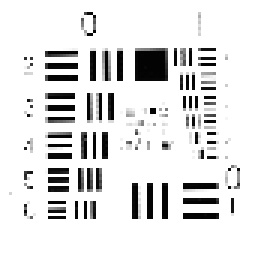
\includegraphics[width=5cm]{fotos/alfanum/k2_1.png} }}
    \qquad
    \subfloat[Método 2]{{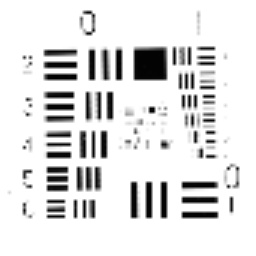
\includegraphics[width=5cm]{fotos/alfanum/k2_2.png} }}
    \qquad
    \subfloat[Método 3]{{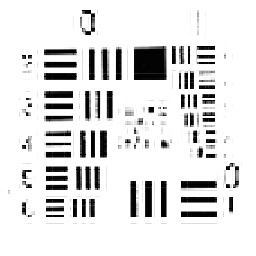
\includegraphics[width=5cm]{fotos/alfanum/k2_3.png} }}
    \caption{Comparación de métodos para $k = 2$}
    \label{fig:example}
\end{figure}

En esta ocasión, el comportamiento sigue los lineamientos generales del caso anterior, con la salvedad de que ninguna de las tres imágenes ya es comprensible. Vemos como el ruido comentado en el caso anterior avanzo rápido en el algoritmo bilineal, para casi difuminar la imagen por completo. En el caso del algoritmo que utiliza splines, se puede empezar a ver un pequeño sombreado alrededor de los bordes de los elementos en la imagen, pero a diferencia del método dos, esta solo se extiende a las cercanías y no avanza por toda la imagen.

Por ultimo, presentamos los resultados para $k=4$:

\begin{figure}[H]
    \centering
    \subfloat[Método 1]{{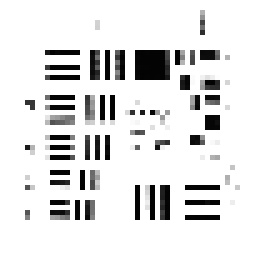
\includegraphics[width=5cm]{fotos/alfanum/k5_1.png} }}
    \qquad
    \subfloat[Método 2]{{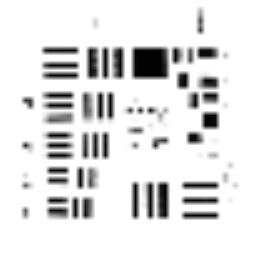
\includegraphics[width=5cm]{fotos/alfanum/k5_2.png} }}
    \qquad
    \subfloat[Método 3]{{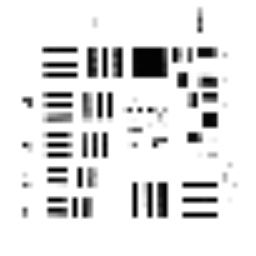
\includegraphics[width=5cm]{fotos/alfanum/k5_3.png} }}
    \caption{Comparación de métodos para $k = 4$}
    \label{fig:example}
\end{figure}

Como era de esperarse las tres imágenes resultantes ya perdieron comprensión en su totalidad. Además, el segundo y tercer método, presentan una alta cantidad de ruido por el difuminado producido respecto de la imagen original.
Queda entonces a la vista una característica que no estábamos considerando hasta entonces en nuestro análisis. El método de los vecinos puede llegar a ofrecer resultados favorables si se cumplen algunas características deseables (nuestra intuición preveía que esta implementación seria superado por los anteriores en cualquier situación) como en este caso. El alto contraste entre las imágenes, hace que en los métodos que introducen cierta correlación o suavizado entre píxeles generen un sombreado que hace mas borrosas las imágenes y que las vuelve menos claras. En contra de nuestros pronósticos, el método de los vecinos podría ser un excelente candidato en estos casos.


\subsubsection{Análisis de los métodos para paisajes}

En esta sección analizamos como se comportan los algoritmos desarrolados para fotos de paisajes. Consideramos una imagen que no presente grandes contrastes como en el análisis anterior y en la que se puedan analizar tanto detalles puntuales (la definición de las ramas del árbol) así como aquellos mucho mas definidos (piedras y ramas que cubren un gran porcentaje de la imagen). Tomamos la siguiente imagen de $256 \times 256$:

\begin{figure}[H]
\centering
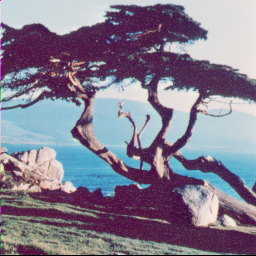
\includegraphics[width=5cm]{fotos/paisaje/orig.png}
\end{figure}

Y reconstruimos la imagen con la metodología ya mencionada en apartados anteriores para $k=1$. Los resultados son los siguientes:

\begin{figure}[H]
    \centering
    \subfloat[Método 1]{{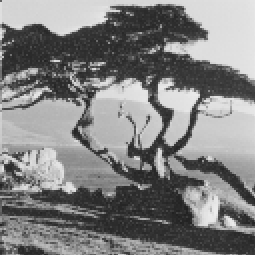
\includegraphics[width=5cm]{fotos/paisaje/k1_1.png} }}
    \qquad
    \subfloat[Método 2]{{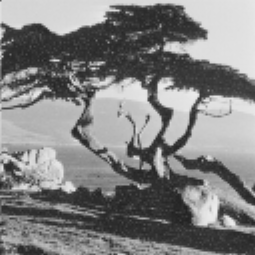
\includegraphics[width=5cm]{fotos/paisaje/k1_2.png} }}
    \qquad
    \subfloat[Método 3]{{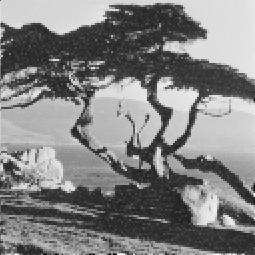
\includegraphics[width=5cm]{fotos/paisaje/k1_3.png} }}
    \caption{Comparación de métodos para $k = 1$}
    \label{fig:example}
\end{figure}

En este primer ejemplo, con un $k$ mínimo, ninguna de las tres imágenes presenta una calidad demasiado desmejorada. 

El $ECM$ y $PSNR$ obtenido para cada uno de los métodos fue el siguiente:
\begin{itemize}
 \item Método 1: ECM de $315.723$ y PSNR de $23.1377$.
 \item Método 2: ECM de $115.114$ y PSNR de $27.5195$.
 \item Método 3: ECM de $332.629$ y PSNR de $22.9112$
\end{itemize}

En particular nos sorprendió ver el ECM de la implementacion que utiliza interpolación por splines, que visualmente esta mas cerca al algoritmo de los vecinos mas cercanos(el cual se perfilaba como el de peor rendimiento de los tres y termino en segundo lugar) que al método dos (de el cual, de hecho, suponíamos era una mejora tanto con el error cuadrático medio como con el PSNR).

En el método 1 puede notarse ya cierto aliasing en los bordes mas prominentes de la fotografía, como el tronco de la izquierda. Además si se observa la sombra de los arboles, que en la imagen originar resultaba uniforme puede verse ahora como el método 1 y 3 introdujo una gran cantidad de ruido en esos lugares.

Ahora lo hacemos para $k=2$, se obtiene esto:

\begin{figure}[H]
    \centering
    \subfloat[Método 1]{{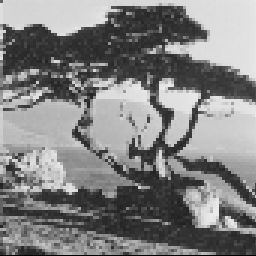
\includegraphics[width=5cm]{fotos/paisaje/k2_1.png} }}
    \qquad
    \subfloat[Método 2]{{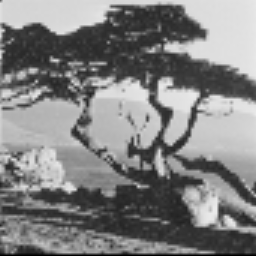
\includegraphics[width=5cm]{fotos/paisaje/k2_2.png} }}
    \qquad
    \subfloat[Método 3]{{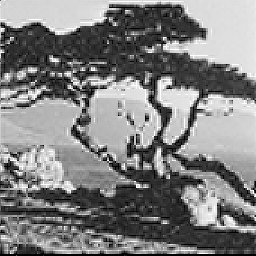
\includegraphics[width=5cm]{fotos/paisaje/k2_3.png} }}
    \caption{Comparación de métodos para $k = 2$}
    \label{fig:example}%
\end{figure}

En este segundo caso, aun con un pequeño cambio en el $k$, podemos apreciar como el método de los vecinos y el de splines (método 1 y 3 respectivamente) empiezan a introducir una gran cantidad de ruido. En el caso del método dos, a diferencia de lo ocurrido durante el análisis de caracteres alfanuméricos, el suavizado que se produce en la imagen si ayuda a que esta se mantenga entendible y el difuminado termina favoreciendo a la comprensión de la misma (esto no ocurría en los caracteres alfanuméricos, porque este mismo suavizado termina oscureciéndola y quitándole claridad).
Una vez mas, los valores de error cuadrático medio y la relación signal/ruido apoyan el análisis realizado e incluso demuestran que la diferencia introducida en el ECM se duplica entre cada método.

\begin{itemize}
 \item Método 1: ECM de $724.517$ y PSNR de $19.5303$.
 \item Método 2: ECM de $293.755$ y PSNR de $23.4509$.
 \item Método 3: ECM de $444.18$ y PSNR de $21.6552$
\end{itemize}

Además la implementación de vecinos mas cercanos 1 presenta un aliasing muy notable en casi toda la imagen.

Ahora lo hacemos para $k=3$, se obtiene esto:
\begin{figure}[H]
    \centering
    \subfloat[Método 1]{{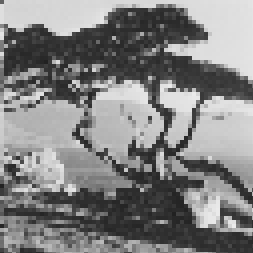
\includegraphics[width=5cm]{fotos/paisaje/k3_1.png} }}%
    \qquad
    \subfloat[Método 2]{{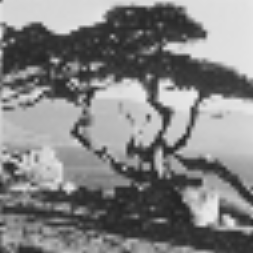
\includegraphics[width=5cm]{fotos/paisaje/k3_2.png} }}%
    \qquad
    \subfloat[Método 3]{{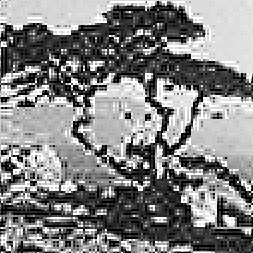
\includegraphics[width=5cm]{fotos/paisaje/k3_3.png} }}%
    \caption{Comparación de métodos para $k = 3$}%
    \label{fig:example}%
\end{figure}

En este caso, podemos ver nuevamente como el aumento mínimo del valor de $k$ produce niveles altísimos de perdida de definición en las tres imágenes. Contraria a nuestra intuición, el método dos sigue ofreciendo un mejor desempeño en este caso, incluso contra el método de Splines. El método de los vecinos, que no presenta ningún suavizado, queda rápidamente relegada al ultimo lugar en cuanto a la cantidad de ruido (Notese como ya es difícil diferenciar las zonas de mayor definición como las ramas del árbol e incluso empieza a estar comprometida nuestra capacidad de diferenciar donde empieza la piedra que se encuentra en la zona media izquierda y donde lo hace la superficie del piso). En el método dos podemos confirmar que, como en el caso anterior, a cambio de introducir cierto sombreado en la imagen se consigue la mejor definición colocándolo nuevamente como el de mejor desempeño.
Una vez mas, los valores de $ECM$ y $PSNR$ son, como era de esperarse, los siguientes:
\begin{itemize}
 \item Método 1: ECM de $1099.83$ y PSNR de $17.7175$.
 \item Método 2: ECM de $400.854$ y PSNR de $22.1009$.
 \item Método 3: ECM de $493.992$ y PSNR de $21.1936$
\end{itemize}
Notese como los métodos dos y tres presentan una pequeña diferencia comparándola con la cantidad de error introducida por el primer método.

Testeamos con un valor extremo de $k$ para ver cuales son los resultados, para $k=10$ se obtiene:

\begin{figure}[H]
    \centering
    \subfloat[Método 1]{{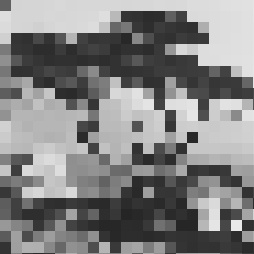
\includegraphics[width=5cm]{fotos/paisaje/k10_1.jpg} }}%
    \qquad
    \subfloat[Método 2]{{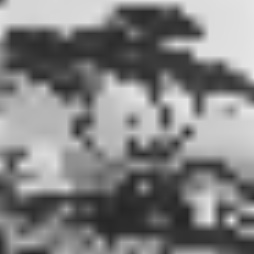
\includegraphics[width=5cm]{fotos/paisaje/k10_2.jpg} }}%
    \qquad
    \subfloat[Método 3]{{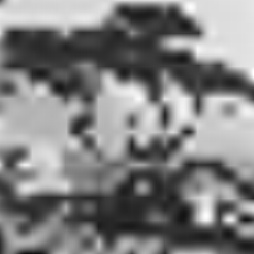
\includegraphics[width=5cm]{fotos/paisaje/k10_3.jpg} }}%
    \caption{Comparación de métodos para $k = 3$}%
    \label{fig:example}%
\end{figure}

Como esperábamos, ninguna de las tres imágenes es ya reconocible. El método uno, vecinos, es claramente el mas perjudicado con una imagen final que recuerda a las viejas imágenes de 8bits debido a su alto grado de aliasing. En el caso del método de splines, la imagen es algo mas clara, sin embargo y contrario a nuestra intuición, a este nivel se observan cierto cuadriculado en la imagen, producto de las ventanas que tomamos para su aproximación. Curiosamente, esperábamos que sea el método Bilineal quien cuente con este desventaja, producto de la falta de suavizado entre los píxeles vecinos.
\begin{itemize}
 \item Método 1: ECM de $2976.63$ y PSNR de $13.3936$.
 \item Método 2: ECM de $1266.65$ y PSNR de $17.1042$.
 \item Método 3: ECM de $1454.78$ y PSNR de $16.5028$
\end{itemize}

Como puede verse, el método 2 continua siendo el que produce menos ECM y el que obtiene mejor PSNR incluso para estos niveles altísimos de $k$.

\subsection{Análisis de los métodos para rostros}


En esta ultima sección analizamos como se comportan los métodos para fotos de rostros. Centraremos nuestro análisis en el comportamiento de los tres algoritmos frente a rasgos particulares del rostro para poder valorar la calidad de los mismos. Tomamos la siguiente fotografía de $256\times 256$:

\begin{figure}[H]
\centering
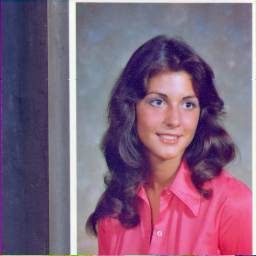
\includegraphics[width=5cm]{fotos/rostro/orig.png}
\end{figure}

Presentamos el mismo análisis que en las imágenes anteriores ($k=1$, $k=2$ y $k=3$)

\begin{figure}[H]
    \centering
    \subfloat[Método 1]{{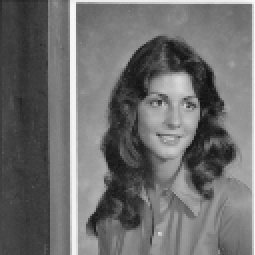
\includegraphics[width=5cm]{fotos/rostro/k1_1.png} }}%
    \qquad
    \subfloat[Método 2]{{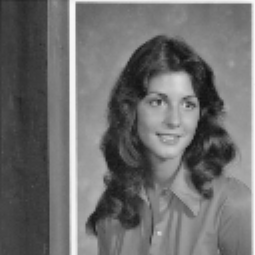
\includegraphics[width=5cm]{fotos/rostro/k1_2.png} }}%
    \qquad
    \subfloat[Método 3]{{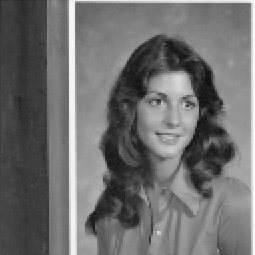
\includegraphics[width=5cm]{fotos/rostro/k1_3.png} }}%
    \caption{Comparación de métodos para $k = 1$}%
    \label{fig:example}%
\end{figure}

ECM y PSNR para $k = 1$:

\begin{itemize}
 \item Método 1: ECM de $95.6087$ y PSNR de $28.3258$.
 \item Método 2: ECM de $32.6121$ y PSNR de $32.997$.
 \item Método 3: ECM de $105.23$ y PSNR de $27.9094$
\end{itemize}

\begin{figure}[H]
    \centering
    \subfloat[Método 1]{{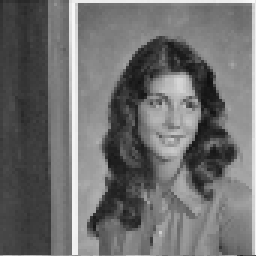
\includegraphics[width=5cm]{fotos/rostro/k2_1.png} }}%
    \qquad
    \subfloat[Método 2]{{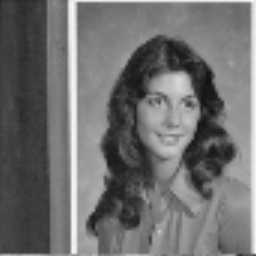
\includegraphics[width=5cm]{fotos/rostro/k2_2.png} }}%
    \qquad
    \subfloat[Método 3]{{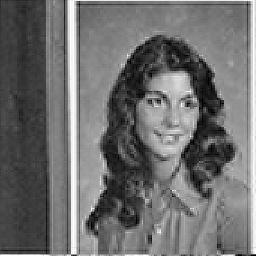
\includegraphics[width=5cm]{fotos/rostro/k2_3.png} }}%
    \caption{Comparación de métodos para $k = 2$}%
    \label{fig:example}%
\end{figure}

ECM y PSNR para $k = 2$:

\begin{itemize}
 \item Método 1: ECM de $235.245$ y PSNR de $24.4156$.
 \item Método 2: ECM de $87.1968$ y PSNR de $28.7258$.
 \item Método 3: ECM de $150.451$ y PSNR de $26.3569$
\end{itemize}

\begin{figure}[H]
    \centering
    \subfloat[Método 1]{{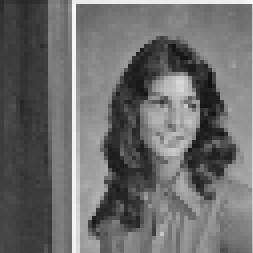
\includegraphics[width=5cm]{fotos/rostro/k3_1.png} }}
    \qquad
    \subfloat[Método 2]{{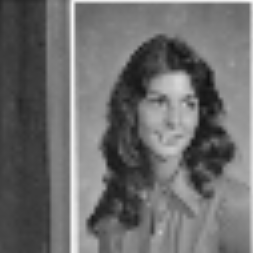
\includegraphics[width=5cm]{fotos/rostro/k3_2.png} }}
    \qquad
    \subfloat[Método 3]{{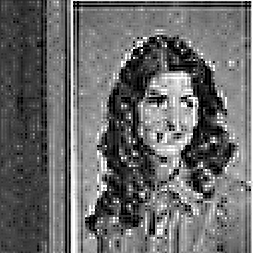
\includegraphics[width=5cm]{fotos/rostro/k3_3.png} }}
    \caption{Comparación de métodos para $k = 3$}
    \label{fig:example}
\end{figure}

ECM y PSNR para $k = 3$:

\begin{itemize}
 \item Método 1: ECM de $389.559$ y PSNR de $22.2251$.
 \item Método 2: ECM de $113.193$ y PSNR de $27.5926$.
 \item Método 3: ECM de $159.421$ y PSNR de $26.1054$.
\end{itemize}

Este análisis vuelve a repetir el mismo comportamiento que vimos en el caso de las imágenes de paisajes en cuanto a la relación entre el error introducido por cada uno de los métodos (aunque con distintos valores, la relación en el fondo es la misma). Sin embargo, y como una apreciación totalmente subjetiva, consideramos que el método tres (aproximación por splines), conserva mucho mejor las características del rostro de la imagen que los otros dos; el primer caso debido a la introducción excesiva de aliasing de la imagen, y el caso tres debido a que, debido al suavizado general de toda la imagen que ya mencionamos en ocasiones anteriores, difumina demasiado los detalles menores del rostro de la imagen.

Testeamos con un valor extremo de $k$ para ver cuales son los resultados, para $k=10$ se obtiene:

\begin{figure}[H]
    \centering
    \subfloat[Método 1]{{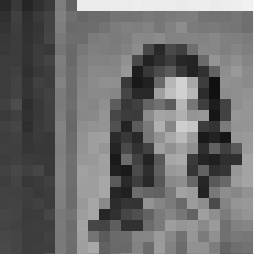
\includegraphics[width=5cm]{fotos/rostro/k10_1.jpg} }}%
    \qquad
    \subfloat[Método 2]{{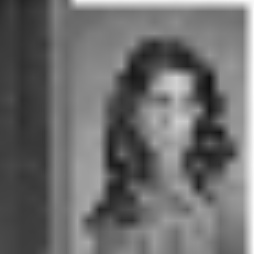
\includegraphics[width=5cm]{fotos/rostro/k10_2.jpg} }}%
    \qquad
    \subfloat[Método 3]{{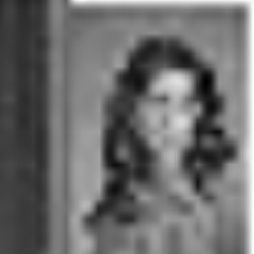
\includegraphics[width=5cm]{fotos/rostro/k10_3.jpg} }}%
    \caption{Comparación de métodos para $k = 3$}%
    \label{fig:example}%
\end{figure}

ECM y PSNR para $k = 10$:

\begin{itemize}
 \item Método 1: ECM de $1563.05$ y PSNR de $16.1911$.
 \item Método 2: ECM de $684.334$ y PSNR de $19.7781$.
 \item Método 3: ECM de $639.892$ y PSNR de $20.0697$
\end{itemize}

Una vez mas, vuelve a repetirse resultados similares que en el caso anterior para $k=10$. De nuevo el método de los vecinos pierde frente a los demás por una gran diferencia (tanto 'visual' como con respecto al ECM y el PSNR). Las diferencias entre el método Bilineal y el método de splines es ,muy pequeña aunque en este caso resulta levemente mejor el método 3.


\subsubsection{Conclusiones del análisis de los métodos}
Como pudimos apreciar a lo largo de los distintos análisis realizados, no existe un método que sea claramente un ganador.
Si bien es cierto que el método dos es el que introduce la menor cantidad de errores, una apreciación mas 'subjetiva' y alejada de los números nos deja las siguientes sensaciones:
\begin{enumerate}
 \item El método de los vecinos puede llegar a mostrar mejores resultados en situaciones de imágenes que consisten en elementos frente a un fondo uniforme con un alto contraste debido a que al no realizar ninguna interpolación entre los píxeles evita introducir sombreados innecesarios.
 \item El método Bilineal, a pesar de ser el mejor en cuanto a errores y la cantidad de ruido introducida en las imágenes, no siempre es considerado el algoritmo óptimo según nuestro análisis. En situaciones donde la imagen presenta regiones de alta cantidad de detalles (como puede ser el rostro de una persona en el caso analizado), genera un sombreado que hace perder definición en estas zonas. Situación que no ocurre para el método de Splines. Sin embargo, en imágenes donde no hay regiones de grandes detalles (como puede ser un paisaje) si lo consideramos el óptimo.
 \item El método de interpolación de Splines, que presenta valores cercanos al mejor candidato (la implementación Bilineal) en la mayoría de los casos, tiene la ventaja de que, al introducir menor cantidad de 'sombreado' que este ultimo, conserva mejor aquellos detalles mencionados en donde el método Bilineal perdía claridad.
\end{enumerate}


% \subsection{Análisis de los metodos}
%Yo diría que esto no va mas

% Empleamos un análisis incremental respecto al valor de los pixeles intermedios introducidos (el valor de $k$) para poder analizar los distintos métodos de forma escalonada y presentar conclusiones mucho más claras. Dado que nuestros algoritmos solo funcionan cuando los valores de las imágenes son divisibles por $k$, no deben asumirse una correlación entre los distintos valores de este debido a que las imágenes a analizar no siempre pudieron ser las mismas.

% \subsubsection{K = 2}
% Nuestro primer análisis se concentra en el valor mínimo de $k$ para el cual esperabamos que el comportamiento de los tres métodos se mantenga bastante estable. Nuestra intuición proviene de la idea de que todos ellos ofrecian una perdida en la calidad de la imagen bastanta pequeña en relación al zoom pedido.
% Como podemos apreciar en los gráficos a continuación, nuestra intuición se corresponde con los valores de $PSNR$, donde los tres métodos se comportan relativamente iguales, sin embargo, nos sorprende ver que para el error cuadrático medio (y para $PSNR$ también, pero en menor medida) la técnica de interpolación Bilineal obtuvo resultados muy destacables (de hecho, casi constantes), incluso frente a la técnica de Splines que esperabamos siempre tenga un mejor rendimiento. La conclusión respecto de este fenómeno se explica al final del artículo.

% \begin{center}
% \includegraphics[scale=0.50]{imagenes/K2PSNR.png}
% \includegraphics[scale=0.50]{imagenes/K2ECM.png}
% \end{center}

% \subsubsection{K = 4}
% Para este segundo caso es cierto que, como esperabamos, el error cuadrático medio del método de los vecinos se dispara rápidamente mientras que los de interpolación bilineal y splines se mantienen prácticamente iguales. Lo mismo sucede para los valores de PSNR, siendo los del método de vecinos los únicos que disminuyen con una diferencia de casi 5 puntos.

% \begin{center}
% \includegraphics[scale=0.50]{imagenes/K4PSNR.png}
% \includegraphics[scale=0.50]{imagenes/K4ECM.png}
% \end{center}

% \subsubsection{K = 6}
% Entrando en valores de $k$ mucho más elevados, nuestro análisis empezó a dejar de coincidir con lo que creiamos en un primer momento serían los resultados finales, debido a que el método de Splines no logró sacar una diferencia notoria frente al de interpolación Bilineal, sino que incluso ambos métodos se mantuvieron prácticamente constantes.  Al momento de obtener los resultados nos llamaron poderosamente la atención los valores de ECM obtenidos para las tres primeras imágenes, pero luego de hacer un análisis en conjunto de estas, llegamos a la conclusión de que la suba desmesurada en estos valores se debe a la elevada variabilidad de los contrastes en la escena (el interior de un hogar muy decorado, la foto aérea de un barrio, etc). 

% \begin{center}
% \includegraphics[scale=0.50]{imagenes/K6PSNR.png}
% \includegraphics[scale=0.50]{imagenes/K6ECM.png}
% \end{center}

% \subsubsection{K = 10}
% Por último, para valores que ya se consideran altos de $k$ el método de interpolación Bilineal todavía sigue desempeñandose igual o incluso a veces levemente mejor que el de Splines. Esto no solo contradice nuestra intuición, sino que debido a la performance de ambos, estos resultados colocan al método de interpolación como el más apto en relación benenficio/tiempo, muy por encima del de Splines (ambos ya muy por encima del método de vecinos a esta altura).

% \begin{center}
% \includegraphics[scale=0.50]{imagenes/K10PSNR.png}
% \includegraphics[scale=0.50]{imagenes/K10ECM.png}
% \end{center}

\subsection{Análisis de tiempos}
El análisis de tiempo, a diferencia del de los métodos, no ofreció ninguna respuesta que no hayamos podido intuir durante la codificación de los algoritmos. Es claro que a medida que el método se perfecciona en la búsqueda de resultados más suaves, también aumenta el tiempo necesario de cálculo.

\begin{center}
\includegraphics[scale=0.50]{imagenes/K2T1.png}
\includegraphics[scale=0.50]{imagenes/K2T2.png}
\includegraphics[scale=0.50]{imagenes/K4T.png}
\includegraphics[scale=0.50]{imagenes/K6T.png}
\includegraphics[scale=0.50]{imagenes/K10T.png}
\end{center}

